\chapter{Brugervejledning og eksempel}

\section{Forestillinger}

\subsection{Åben Bookie}

Når "Bookie" bliver kørt, kommer man direkte ind på programmets brugergrænseflade. Dog er det ikke muligt at se salene, da der indtil videre ikke er blevet valgt nogen forestilling. Forestillingerne har et forhold til salene, men ikke omvendt. \ref{screenshot: bookie} viser Bookie's startside, hvor der også er muligt at se feltet, hvor ekspedienten kan indtaste kundens telefonnummer og derefter reservere billetter. Dette kan dog først gennemføres efter at en forestilling er valgt. 

\begin{figure}[h]
  \centering
  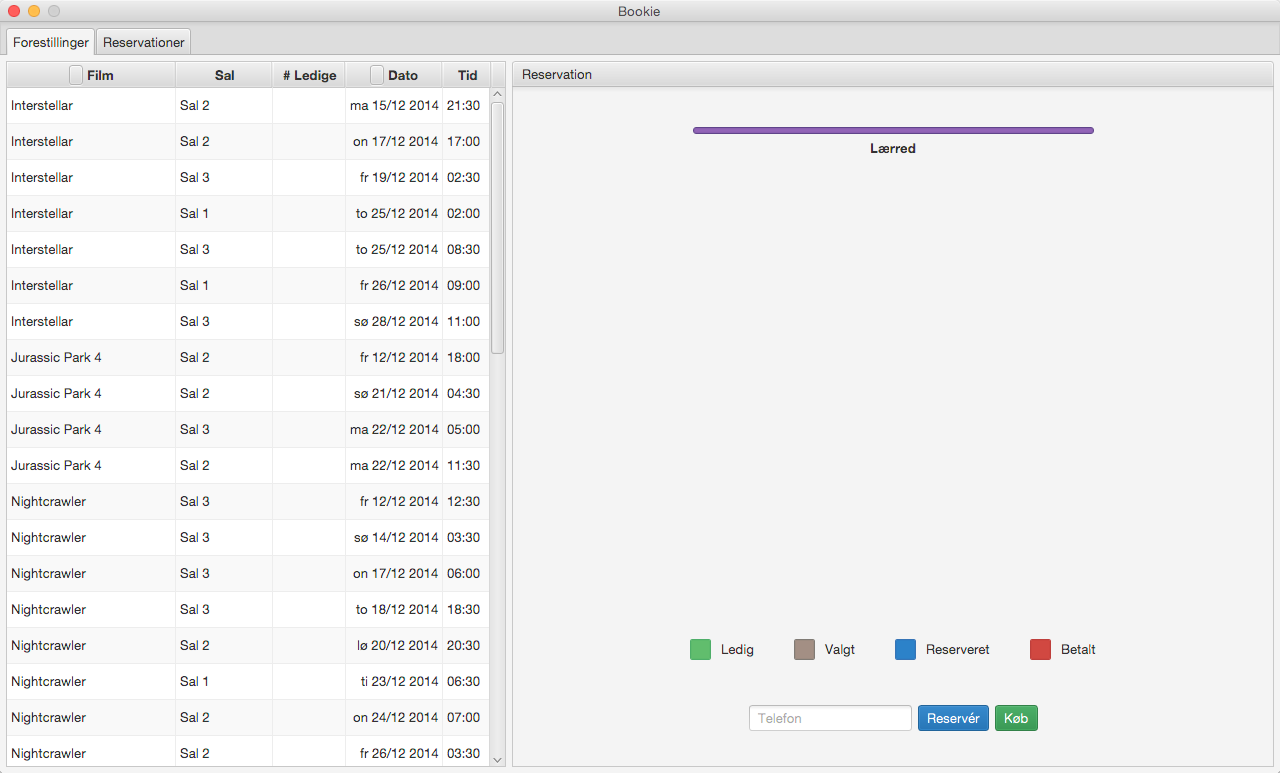
\includegraphics[width=\textwidth]{bookie.png}
  \caption{Bookie startside}
  \label{screenshot: bookie}
\end{figure}

\subsection{Vælg forestilling}

Der er muligt at sortere efter hvilken film kunden vil se, hvilken sal han/hun vil se den i eller hvilken dag/tidspunkt. Uanset hvilken ønske kunden har, så kan ekspedienten hurtigt og nemt trykke på baren med den ønskede kolonne, hvorefter det valgte element bliver sorteret.

I dette eksempel er der blevet sorteret efter film, hvorefter der er blevet valgt en forestilling (\ref{screenshot: chosen-showtime}), og det er nu muligt at se den tilhørende sal med tilhørende sæder.

\begin{figure} [h]
  \centering
  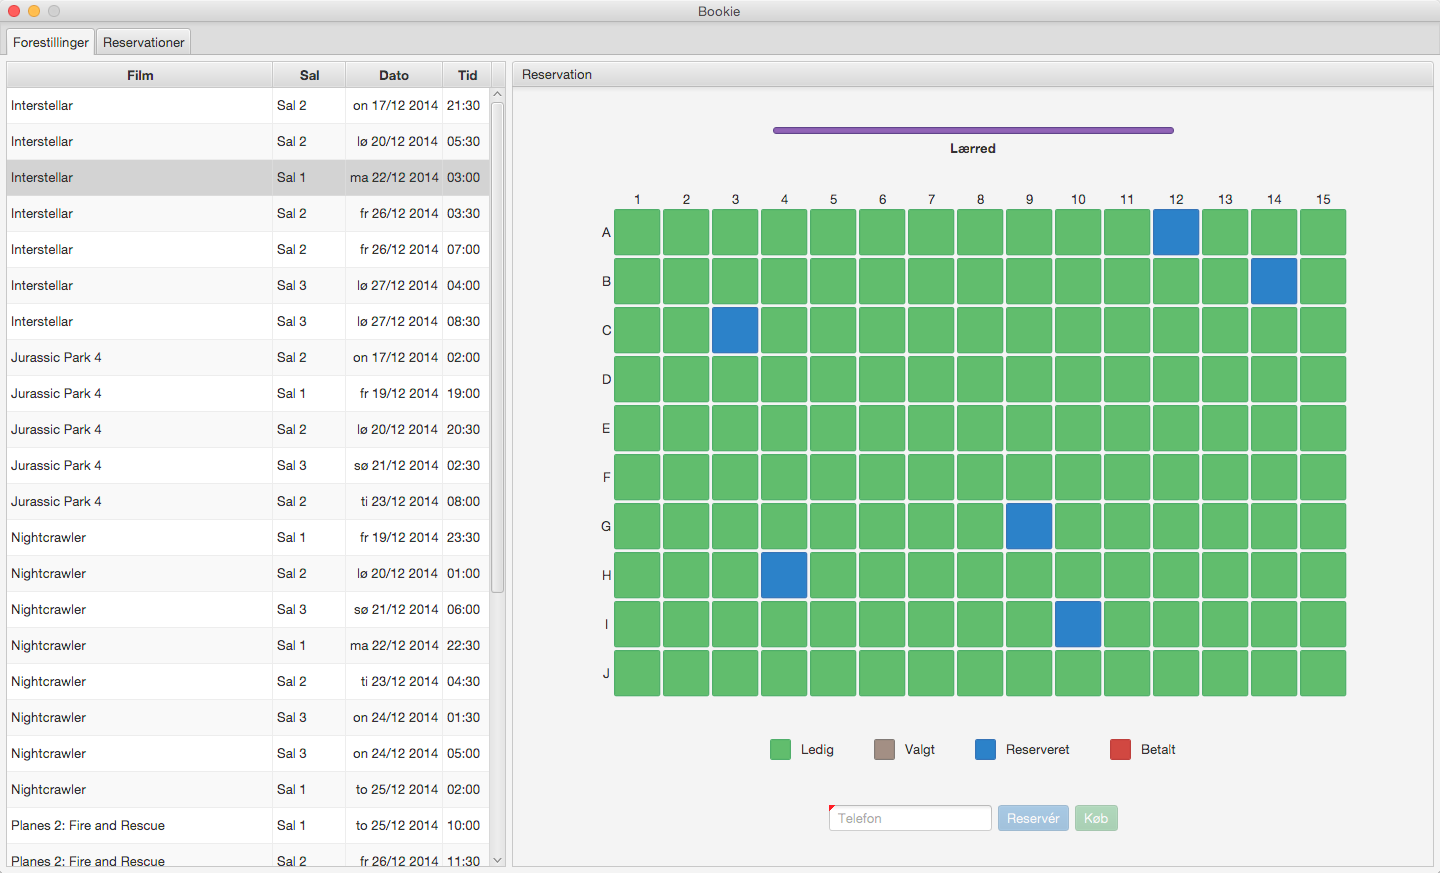
\includegraphics[width=\textwidth]{chosen-showtime.png}
  \caption{Den valgte forestilling: Interstellar}
  \label{screenshot: chosen-showtime}
\end{figure}

\subsection{Vælg sæder}

Sæderne er angivet i rækker og kolonner, hvor rækkerne har fået navne efter alfabetet og kolonnerne efter tal. Dette gør det meget nemt at beskrive hvor i salen de valgte sæder befinder sig. Holder ekspedienten musen hen over et af de grønne sæder, og trykker på det, resulterer det i at sædet får en grå farve (dette kan også ses i legenden i \ref{screenshot: chosen-seats1}).

\begin{figure} [h]
  \centering
  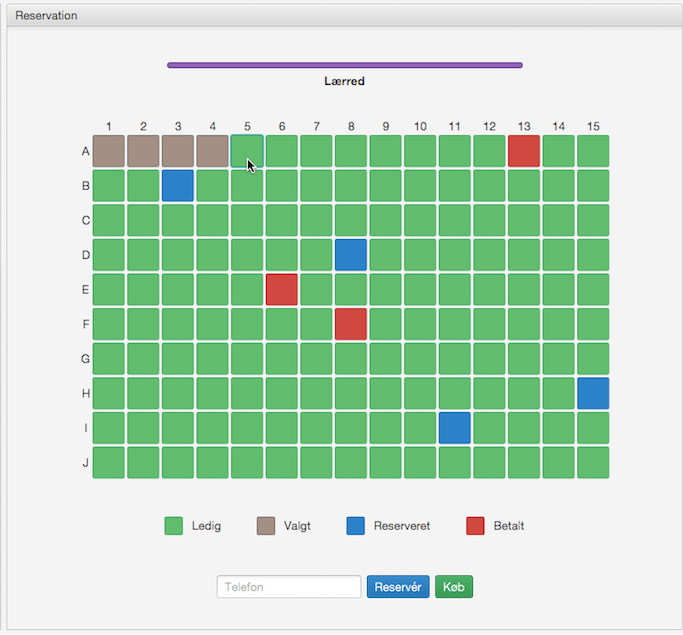
\includegraphics[width=0.4\textwidth]{chosen-seats1.png}
  \caption{Valgte sæder}
  \label{screenshot: chosen-seats1}
\end{figure}

\subsection{Indtast telefonnummer}

Efter at sæderne er blevet valgte, er det muligt at indtaste et telefonnummer (\ref{screenshot: phone-number1}). Trykker man derefter på \textit{Reservér} knappen, ændrer sæderne farve og bliver blå. Hvilket viser ekspedienten, at reservationen er gennemført. Ses også i \ref{screenshot: booked-seats1}

\begin{figure} [h]
  \centering
  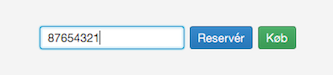
\includegraphics[width=0.4\textwidth]{phone-number1.png}
  \caption{Telefonnummer bliver indtastet.}
  \label{screenshot: phone-number1}
\end{figure}

\begin{figure} [h]
  \centering
  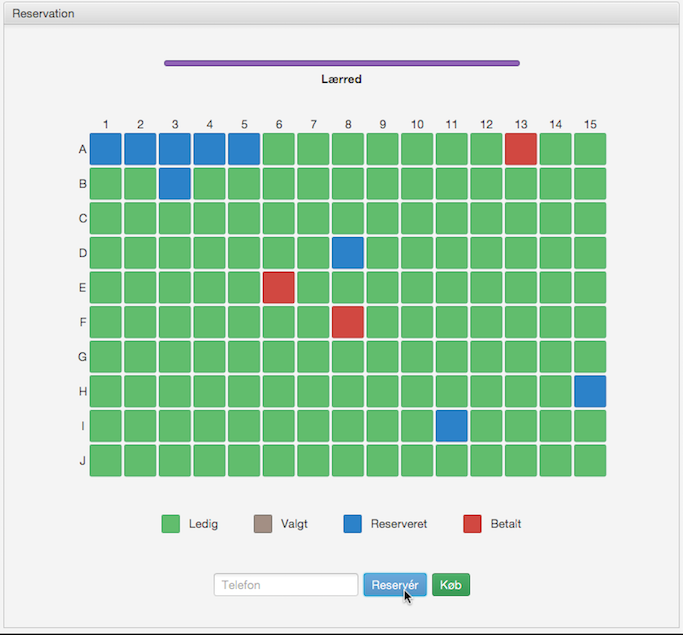
\includegraphics[width=0.4\textwidth]{booked-seats1.png}
  \caption{Reserverede sæder.}
  \label{screenshot: booked-seats1}
\end{figure}

\section{Reservationer}

\subsection{Gå til Reservationer}
Efter at sæderne er reserverede, er der blevet oprettet billetter inde i Reservationer. Alle de eksisterende reservationer kan ses inde på \textit{Reservationer} oppe i venstre hjørne (\ref{screenshot: go-to-reservations1}). Her er også muligt at redigere eller slette dem.

\begin{figure} [h]
  \centering
  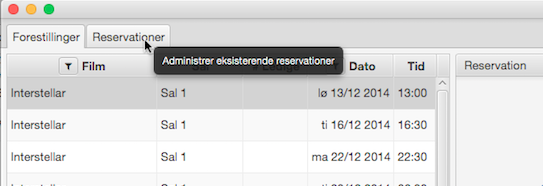
\includegraphics[width=0.4\textwidth]{go-to-reservations.png}
  \caption{Gå til alle reservationer.}
  \label{screenshot: go-to-reservations1}
\end{figure}

\subsection{Filtrering af telefonnumre}

Øverst i venstre hjørne af denne side er der et felt til filtrering af telefonnumre (\ref{screenshot: filter1}).

\begin{figure} [h]
  \centering
  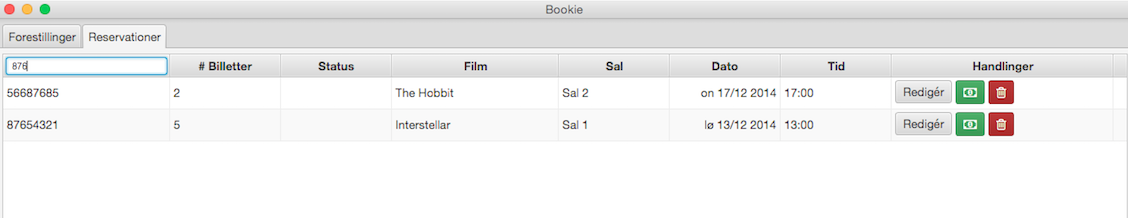
\includegraphics[width=0.4\textwidth]{filter1.png}
  \caption{Filtrering af numre.}
  \label{screenshot: filter1}
\end{figure}
